\documentclass[10pt]{article}

\usepackage{spheric}
%%%TITLE
\title{Numerical Simulation of the Damage of Multi-floor Buildings by Conical Projectile With SPH Method}
\date{}

%%AFFILIATIONS
\author[$\relax$]{Qiang Hong-fu}
\author[$\relax$]{Sun Xin Ya}
\author[$\relax$]{Chen Fu-zhen}
\author[$\relax$]{Zhang Guo Xing}

\affil[$\relax$]{Department of Power Engineering, Xi'an Hi-Tech Institute, China)}

\affil[$\relax$]{\email{}{1430167246@qq.com}}


%%DOCUMENT
\begin{document}

\maketitle

%\SelectedTopics{}

%%PLEASE PUT YOUR ABSTRACT HERE
\begin{abstract}
In the modern war, it is an important means to win the war by effectively breaking the enemy important military facilities, such as the command center of the ground floor. Based on SPH method with fully variable smoothing lengths, the HJC constitutive model and SDPH method are used to deal with the deformation and damage of concrete slab under impact load and the free scattering of dead concrete particles, and the numerical simulation of the process of striking the multi-floor building. The damage degree of multi-floor buildings under different speed and penetration angles is analyzed, and the damage calculation and evaluation model of high-speed penetration of multi-storey buildings is established. Through the theoretical analysis, it is reasonable to show that the numerical simulation results are reasonable, which has some guiding value for predicting the impact performance of the missile and the effective fire strike.


\begin{figure}[!htb]
\centering
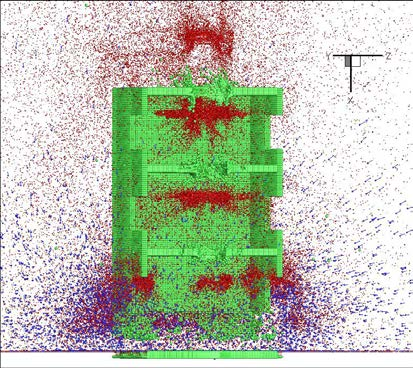
\includegraphics[width=0.6\textwidth]{37-1.png}
\caption{Collapsing of multi-floor buildings after penetrated and impact}\label{fig:37}
\end{figure}

\end{abstract}


%%THE END OF ABSTRACT

\addbib

\end{document}
